\documentclass{standalone}
\usepackage{tikz}
\usetikzlibrary{positioning}
\usetikzlibrary{calc}
\usetikzlibrary{fit}
\usetikzlibrary{shapes}
\usetikzlibrary{arrows}
\usetikzlibrary{intersections}

\tikzset{>=latex}
\tikzset{transaction/.style={font=\small{#1}}}
\tikzset{key/.style={rectangle, draw, minimum height=10pt, text width=2cm, align=center}}
\tikzset{hash/.style={rectangle, draw, minimum height=10pt, text width=1cm, align=center}}
\tikzset{signature/.style={rectangle, draw, minimum height=10pt, text width=2cm, align=center}}

\tikzset{block/.style={font=\small{#1}}}
\tikzset{blockheader/.style={font=\small{#1}}}
\tikzset{field/.style={rectangle, draw, minimum height=10pt, text width=2cm, align=center}}
\tikzset{hash/.style={rectangle, dashed, draw, minimum height=10pt, text width=1.2cm, align=center}}
\tikzset{tx/.style={rectangle, draw, minimum height=10pt, text width=2cm, align=center}}


\begin{document}
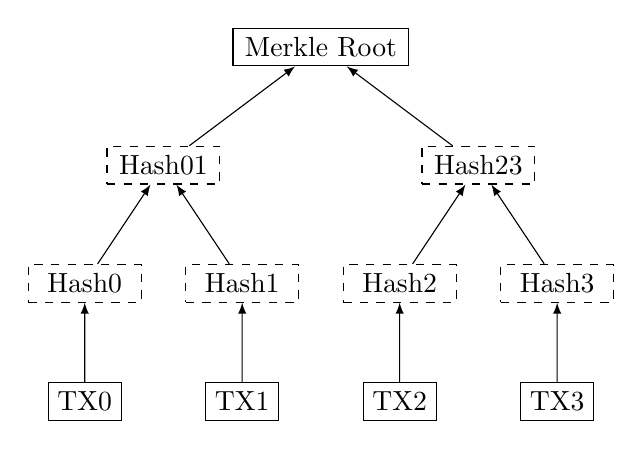
\begin{tikzpicture}[remember picture, every node/.style={},
        level 1/.style={sibling distance=40mm},
        level 2/.style={sibling distance=20mm},
        edge from parent/.style={draw,latex-}
    ]

    \node [field] (merkleRoot0) at (20,20) {Merkle Root}
        child {node [hash] {Hash01}
            child {node [hash] (hash0) {Hash0}
                child {node [grow=down, draw] (tx0) {TX0}}
            }
            child {node [hash] {Hash1}
                child {node [grow=down, draw] {TX1}}
            }
        }
        child {node [hash] {Hash23}
            child {node [hash] {Hash2}
                child {node [grow=down, draw] {TX2}}
            }
            child {node [hash] (hash3) {Hash3}
                child {node [grow=down, draw] {TX3}}
            }
        };

\end{tikzpicture}
\end{document}
